
\documentclass[journal, onecolumn, 11pt]{IEEEtran}
              
\usepackage{graphicx}
\usepackage{subcaption}
\usepackage{booktabs}
\usepackage{multirow}
\usepackage{hyperref}

\begin{document}

\title{Momomood rhythms analysis}

\maketitle

\section{Structure}

\begin{enumerate}
    \item \textbf{Sensor Analysis}

    \begin{itemize}
        \item \textit{Descriptive Statistics}
        \begin{itemize}
            \item Do Patients and Controls differ significantly in their communication and phone usage frequencies?
        \end{itemize}

        \item \textit{Intra-difference in Patterns}
        \begin{itemize}
            \item How consistently does an individual maintain their patterns over time?
        \end{itemize}

        \item \textit{Inter-difference in Patterns}
        \begin{itemize}
            \item How does an individual's pattern deviate from the average pattern of their respective group?
            \item Are communication patterns within the patient group more homogeneous compared to those within the control group?
        \end{itemize}

        \item \textit{Outlier Analysis}
        \begin{itemize}
            \item Who stands out with distinct communication patterns?
            \item Is there a correlation between pattern variability and an individual's well-being?
        \end{itemize}

        \item \textit{Replicability}
        \begin{itemize}
            \item Can the same findings be replicated in the pilot study?
        \end{itemize}
    \end{itemize}
\end{enumerate}


        
\section{Methods}

\subsection{Calls/SMS/Screen Analysis}

In the analysis of Calls, SMS, and Screen data, the battery data served as an effective proxy for compliance. The starting point of the sampling period is designated by the initial battery record, with a total span set to 8 weeks. To neutralize the half-day effect, records from both the first and the last day were systematically excluded. In cases where the frequency was set to 'daily', the sampling commenced at the 00-hour mark. For a 'weekly' frequency, any records that failed to complete an entire week were dismissed. Further filtering excluded participants who yielded less than the 8-week data threshold.

The niimpy toolkit was used for the process of rhythm extraction. Events spanning Calls, SMS, and Screen domains were then aggregated into 1-hour bins, which were subsequently normalized. This normalization process resulted in 24 bins for daily frequencies and 168 bins for weekly frequencies.

We define rhythm consistency as a metric to measure the regularity of those events, quantified as the cosine distance between the average distributions of events in each day. Inter-group variations in rhythm were depicted using a matrix format. Specifically, the matrix cell at position ${ij}$ showcased the cosine distance between subjects $i$ and $j$ from the same group. The overarching objective here was to juxtapose the similarity profiles of members within the same group to those from differing groups. As for intra-group variations, the average cosine distance between consecutive days represented the short-term consistency. In contrast, the long-term consistency was discerned as the cosine distance between a single day and an individual's holistic average over the entire period.

Further analyses included specific controls and checks. An occupation control ensured that the data analysis was limited only to participants who adhered to a Monday-to-Friday work routine. Outlier analysis was then performed by selecting a set of $n$ subjects, specifically those with the most deficient consistency levels, and comparing them against corresponding mood metrics. Lastly, to validate the robustness of our findings, checks were made to ensure the results remained consistent across different binning resolutions, including both 1H and 4H.

\subsection{Actigraphy Analysis}

When dealing with actigraphy data, the original records, which were sampled in 30-second epochs, were resampled to fit into 1-minute epochs for the scope of this study. The definition of sleep phases played a pivotal role in our analysis. The onset of sleep was demarcated by the initiation of a specific, continuous duration of diminished activity. This was typically characterized by durations such as 1, 3, 5, 10, 15, or 20 minutes wherein activity was registered below a predetermined threshold or marked as sleep. Conversely, sleep offset was identified as the last minute within a similar, uninterrupted duration during which a subject was logged as asleep. For our study's purposes, we anchored our choice on a 3-minute threshold to define sleep time and a 5-minute threshold to represent wake time, a decision inspired by prevalent practices in the field.

Activity intervals were classified under three overarching categories: 'ACTIVE', indicative of probable activity; 'REST', symbolizing likely rest; and 'REST-S', which suggested the likelihood of sleep. These data, sampled every 30 seconds, were subsequently resampled to 1-minute intervals. The aggregate of this data was then employed to pinpoint precise status transitions. For instance, a switch from an 'ACTIVE' state to a 'REST' state, followed by a transition to 'REST-S', and finally reverting to 'ACTIVE'. Transitions followed specific rules: a consistent 'REST-S' state over 3 consecutive minutes marked the onset of sleep at the initial timestamp; a 3-minute persistence of the 'REST' state determined the rest onset, while a continuous 5-minute 'ACTIVE' state signaled the offset of sleep. To ensure data coherence, especially concerning sleep records, the day's data was shifted by a full 12 hours, ensuring sleep records remained within the confines of a single day.

\section{Results}

\subsection{Statistics}

The initial dataset contained 151 participants: 30 controls and 121 patients. After applying the data availability criteria, 63 patients and 16 controls remained. Patients had an average age of 34.9 ($\pm$ 12.2) years, while the average age for controls was 38.1 ($\pm$ 14.5) years. Among these participants, there were 15 male and 48 female patients, while the control group consisted of 12 females and 4 males.

In \autoref{tab:desc_events}, we present descriptive statistics of events data collected after the filtering process displayed above.

% Please add the following required packages to your document preamble:
% \usepackage{booktabs}
% \usepackage{multirow}
\begin{table}[htbp]
\centering
\begin{tabular}{@{}clllll@{}}
\toprule
& & \multicolumn{2}{c}{\textbf{Control}} & \multicolumn{2}{c}{\textbf{Patient}} \\
\cmidrule(lr){3-4} \cmidrule(lr){5-6}
\textbf{Feature} & & \textbf{Mean} & \textbf{SD} & \textbf{Mean} & \textbf{SD} \\
\midrule
\multirow{4}{*}{\textbf{Call}} & Outgoing count & 1.26 & 1.22 & 1.59 & 1.38 \\
& Incoming count & 0.67 & 0.58 & 1.27 & 1.17 \\
& Outgoing duration & 5.55 & 5.48 & 7.67 & 9.94 \\
& Incoming duration & 4.87 & 6.08 & 7.89 & 7.36 \\
\midrule
\multirow{2}{*}{\textbf{SMS}} & Outgoing count & 0.67 & 0.99 & 0.95 & 1.27 \\
& Incoming count & 1.24 & 0.79 & 1.48 & 1.23\\
\midrule
\multirow{4}{*}{\textbf{Screen}} & On count & 70.03 & 43.56 & 64.93 & 38.81 \\
& On duration & 72.58 & 66.92 & 86.77 & 101.27 \\
& Use count & 39.41 & 21.94 & 36.62 & 21.73 \\
& Use duration & 225.79 & 116.81 & 181.18 & 129.41 \\
\bottomrule
\end{tabular}
\caption{Communication and screen events: Statistics description. Duration is in minute unit.}
\label{tab:desc_events}
\end{table}


\subsection{Viz of daily/weekly rhythms}

A simple visualization of how distributions of events look like.

\begin{figure}[htbp]
    \centering
    \begin{subfigure}[b]{0.75\textwidth}
        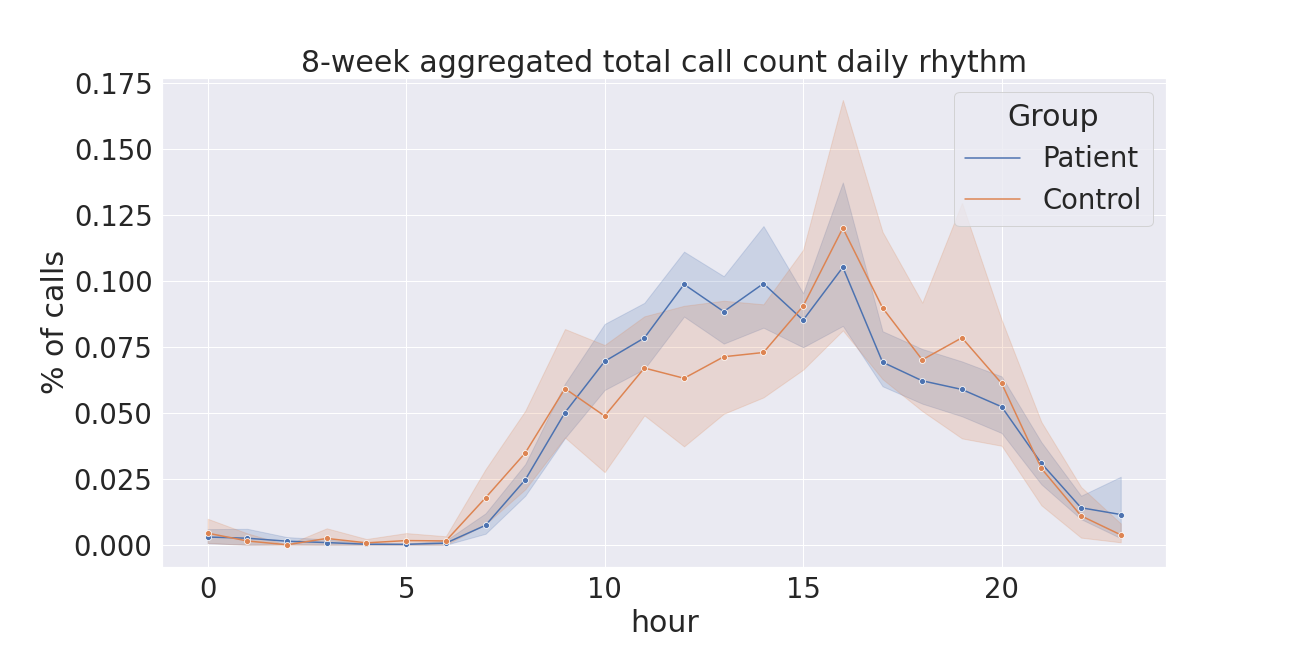
\includegraphics[width=\textwidth]{figs/agg_total_call_rhythm.png}
    \end{subfigure}
    \vfill % To add space between the subfigures
    \begin{subfigure}[b]{0.75\textwidth}
        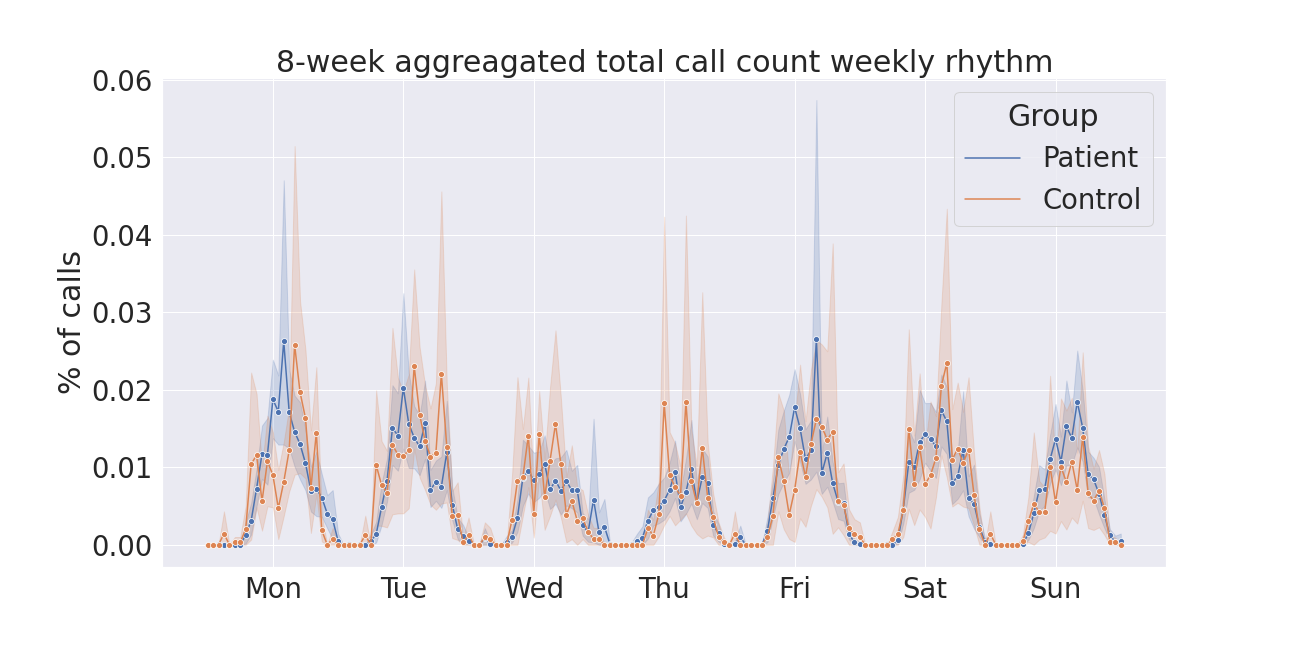
\includegraphics[width=\textwidth]{figs/agg_total_call_count_weekly.png}
    \end{subfigure}
    \caption{Aggregated Daily and Weekly Rhythms.}
\end{figure}

\pagebreak
\subsection{Descriptive analysis}

\begin{figure}[htbp]
    \centering
    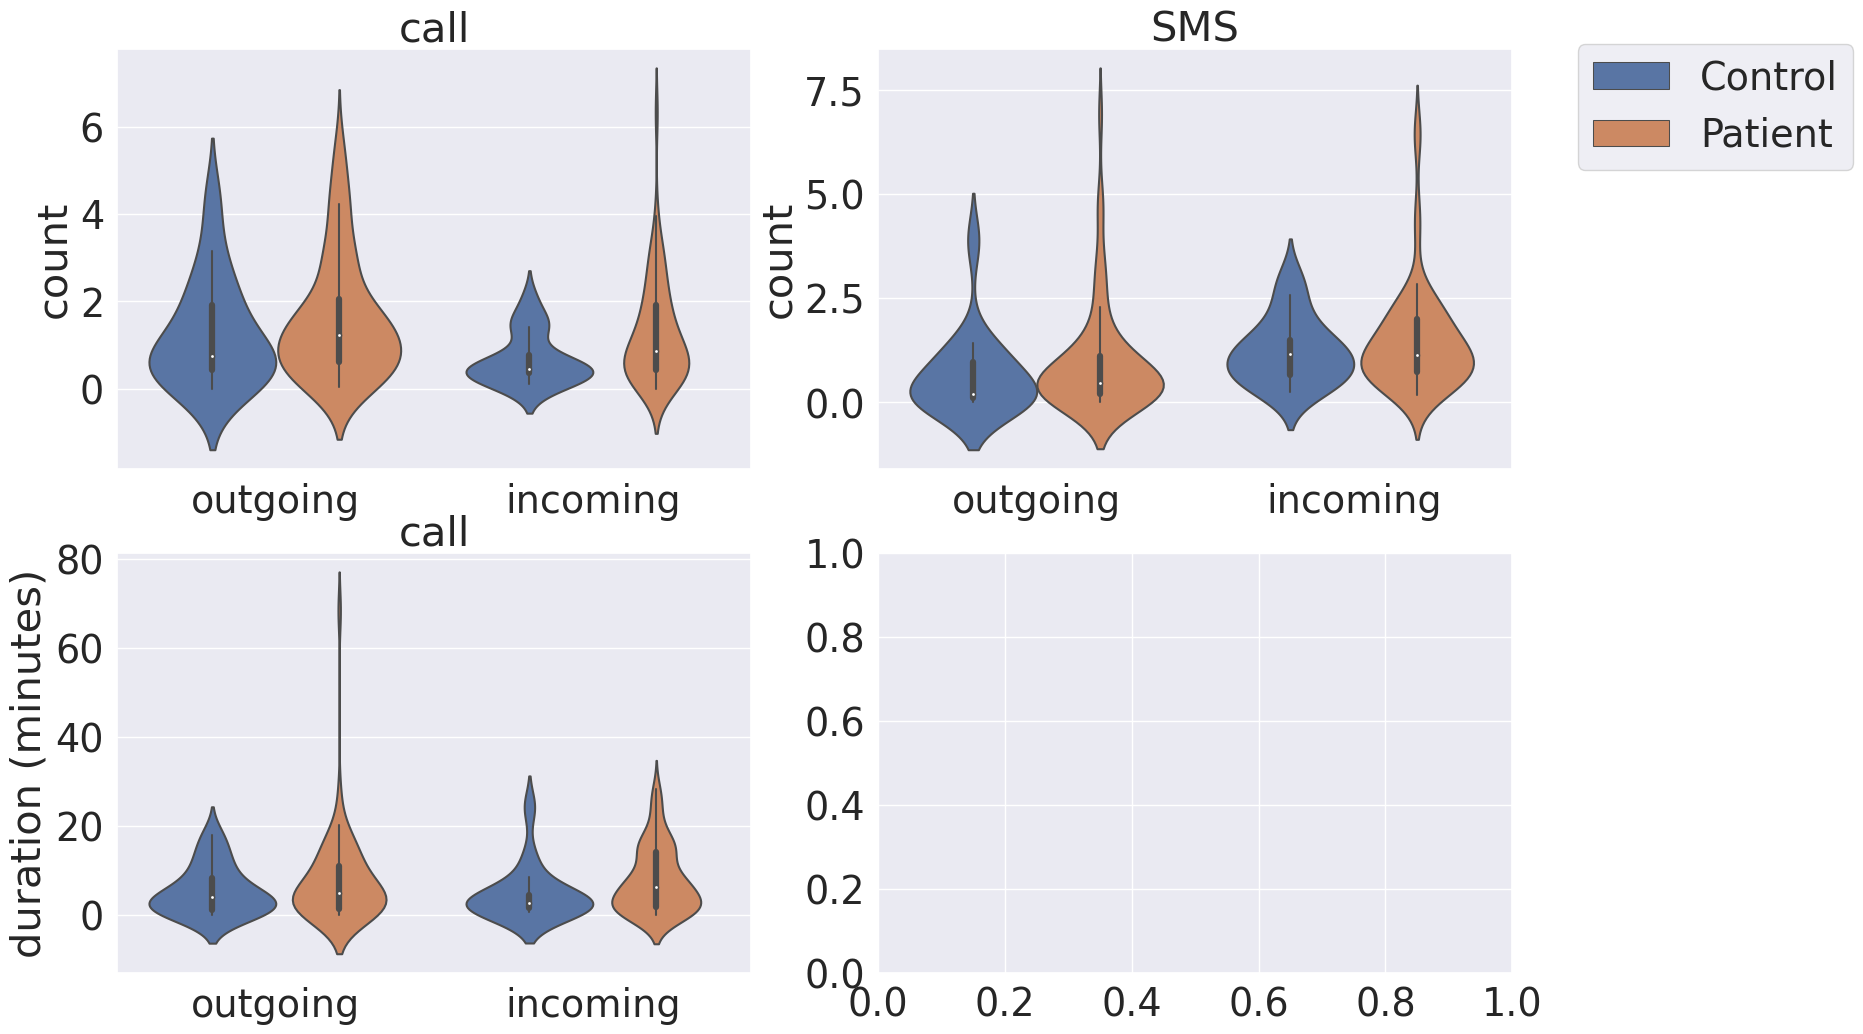
\includegraphics[width=\textwidth]{figs/1_descriptive_comm.png}
    \caption{Descriptive statistics of communications}
\end{figure}

We visualize the overall communications variable here. MWU test was conducted to examine mean difference between group. No significant results were found for all variables.

\begin{figure}[htbp]
    \centering
    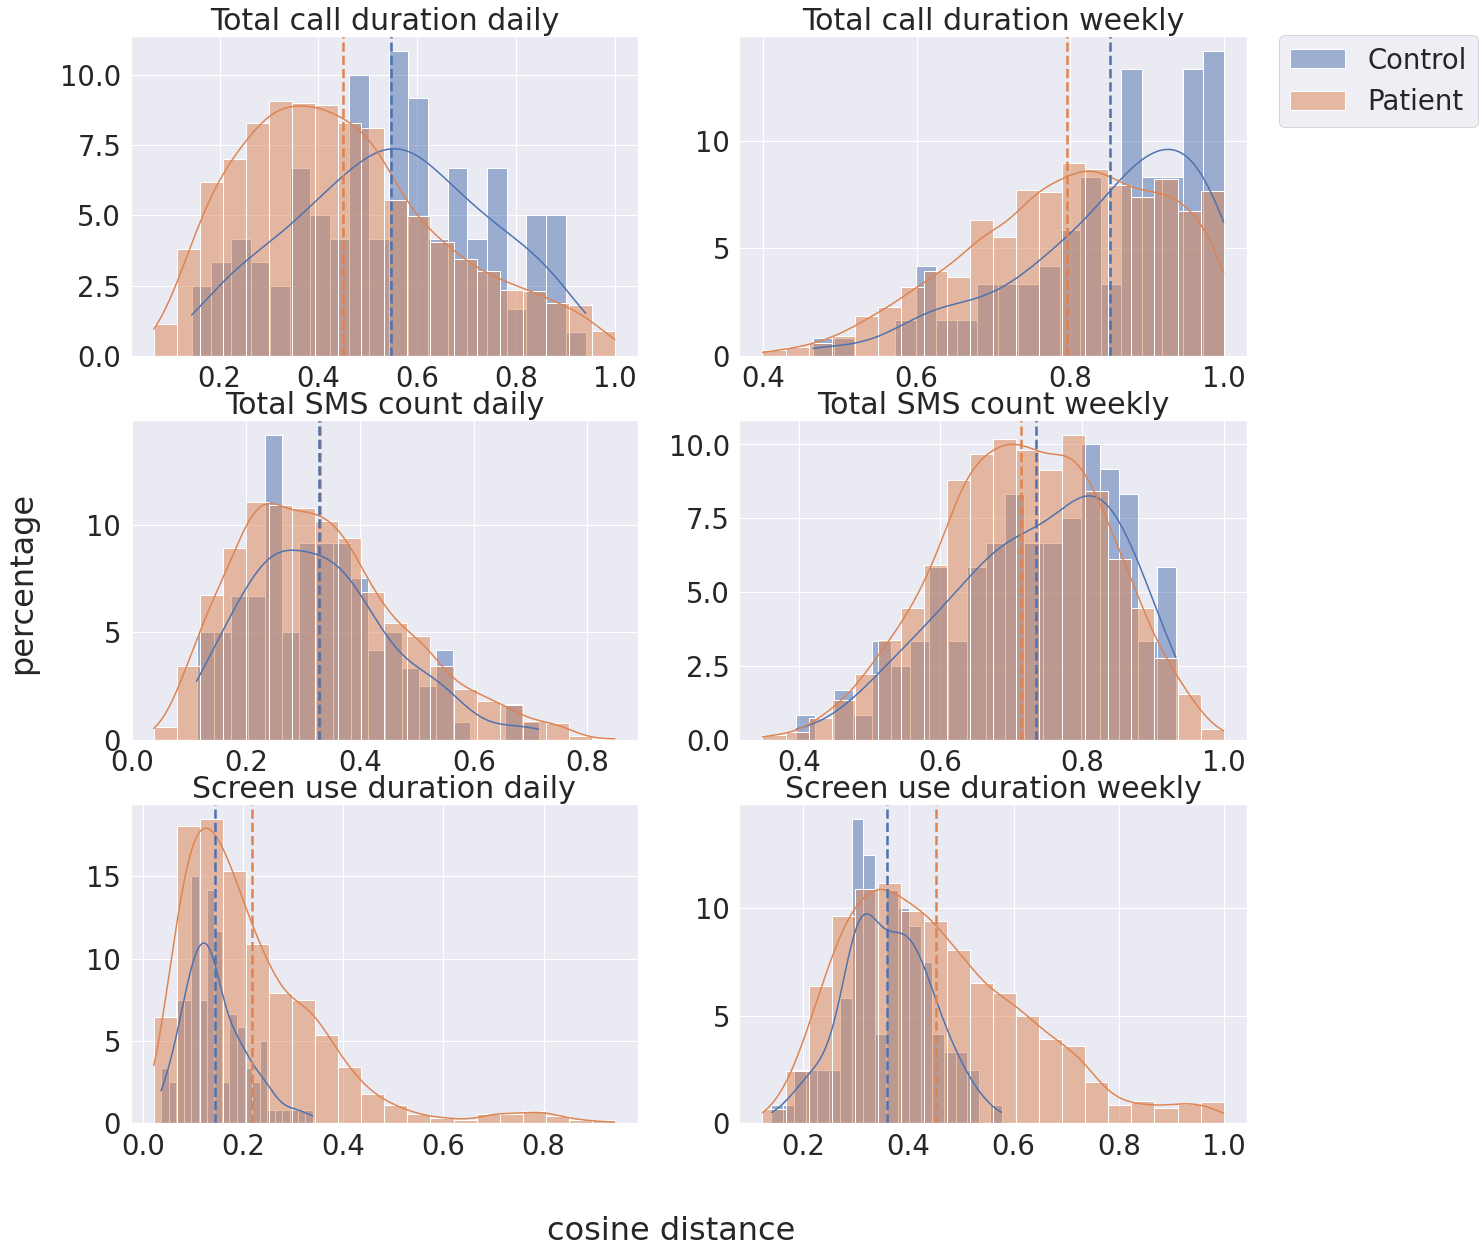
\includegraphics[width=\textwidth]{figs/2_histograms_of_distances.png}
    \caption{PLACEHOLDER: JUST PUT THE PLOT HERE TO SEE HOW IT LOOKS}
\end{figure}

APPLICATIONS:

- Need to check if the code to extract app count and duration actually works. 

- Reasons:

    - App use Duration is computed as the difference in time between two consecutive notifications (?)
    
    - It might not be an indicator of app use, because notification indicates that the phone is put in background.

    - The most reliable source of trust is the foreground information (whether an app is on the foreground). I did not see this info from the database.

\end{document}


\subsection{Occupation control}

\subsection{Outlier analysis}

\bibliographystyle{IEEEtran}
\bibliography{bibtex/blib}

\end{document}